\chapter{Numerical Method}
\label{sec:methods}
In the previous chapter, the basics of plasma physics and the mathematical tools required to analyze plasma dynamics were introduced. Solving the equations of motion for the millions of plasma particles analytically is impractical, this section will outline the Particle-in-Cell (PiC) algorithm as a framework for computer simulation of plasma. A method for implementing photoelectron emission from conducting surfaces is emphasized. First, a general description of the PiC algorithm is introduced as well as the stability criteria of the algorithm. Then the implementation of the PiC algorithm in the PINC framework is discussed with emphasis on the implementation of object charging in plasma. Finally, a method for implementing photoelectron emission into the PINC object module is presented.

\section{Particle In Cell algorithm}
The particle in cell algorithm is a method used in computational plasma physics to analyze large systems of many particles in a computationally efficient manner. This is achieved by the introduction of super particles, computational particles, that represent many real particles as well as by interpolating the forces acting on these super particles to a spatial grid.\\
There are three main ways of simulating the forces acting on a system particles. The particle-particle method (PP) where forces are computed between individual particles. The particle-mesh method (PM) where the forces between the particles are computed as field quantities on the spatial mesh. And the particle-particle-mesh method (PPPM or $P^3M$), which is a combination of the two earlier methods.\\
By far the simplest method computationally is the PP method. However, since all forces between each individual pair of particles is computed, the method is also the most computationally expensive. If the system of interest contains $N_p$ particles, then the number of operations scale as $\mathcal{O}(N^2_p)$ \insertref{Hockney and eastwood p20}. It is therefore impractical to use the PP method for all but the simplest systems, even on highly parallel High Performance Computers (HPC) available today.\\
The PM method computes the forces of a system as field quantities, first by assigning the charges in the system to the mesh by some method, then solving Poisson's equation on the mesh, then computing the forces on the mesh points and interpolating to the individual particles. This method is therefore faster, but usually not as accurate as computing the forces on all particle pairs directly. With $N_g$ grid points, the complexity of this method scales as $\mathcal{O}(N_g \log{N_g})$ thus making this method much more applicable to larger systems than the PP method.

\begin{figure}[h!]
    \centering
    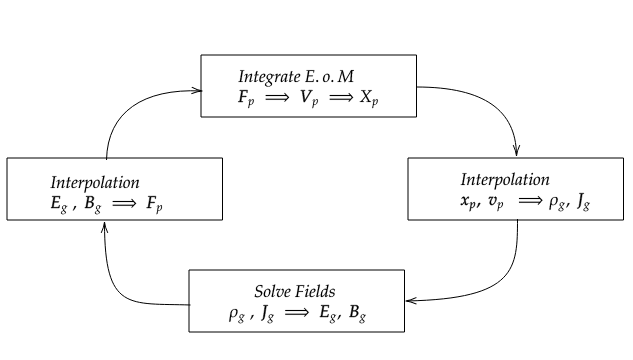
\includegraphics[scale=0.6]{figures/PiC.png}
    \caption{Particle in cell compute cycle}
    \label{fig:pic}
\end{figure}

The PiC algorithm is an example of the PM method, figure \ref{fig:pic} gives an overview of a computational cycle for each time step in the PiC algorithm. Beginning at the box on the right in the figure, a distribution of $N_p$ particles with position $\vb{x}_p$ is interpolated to get the charge $\rho_g$ and current density $\vb{J}_g$ at the surrounding grid points. The two most common methods for this interpolation is the Nearest Grid Point (NGP) scheme, and Cloud in Cell (CIC) scheme.\\
Once the charge and current densities are known on the grid, the next step is to solve for the $\vb{E}$ and $\vb{B}$ fields. This is accomplished by solving Maxwell's equations at the grid points

\begin{subequations}
    \begin{align}
        Gauss's\; Law: \nabla \cdot \vb{E} &= \frac{\rho}{\epsilon_0} \label{eq:gauss} \\
        Gauss's\; Law\; for\; magnetism: \nabla \cdot \vb{B} &= 0 \\
        Maxwell - Faraday's\; equation: \nabla \cross \vb{E} &= - \pdv{\vb{B}}{t}\\
        Ampere's\; Law: \nabla \cross \vb{B} &= \mu_0 \left(\vb{J} + \epsilon_0 \pdv{\vb{E}}{t} \right)
    \end{align}
\end{subequations}

Where $\rho$ is the charge density, $\epsilon_0$ is the vacuum permittivity, $\mu_0$ is the vacuum permeability, and $\vb{E}$ and $\vb{B}$ are the electric and magnetic fields respectively. With the electric and magnetic field computed at the grid nodes, the force on each super particle is computed from Lorentz's force equation and interpolating back to the position of the super particles. Using some numerical integrator the new position and velocity of the super particle is updated from the computed forces, and the cycle can then be repeated for the next time step. 

\section{Particle in Cell implementation in PINC}
In this section, we discuss the methods implemented in PINC that are required for the main PiC compute cycle described in figure \ref{fig:pic} with focus on the particular schemes used in this thesis. The scheme used in PINC for integrating the equations of motion are presented, followed by the multigrid field solver, and finally the particle weighting scheme is discussed. PINC is the work of many researchers, but have been mainly implemented by Sigvald Marholm as part of his Ph.D thesis \insertref{Sigvald's thesis}, Gullik Killie \insertref{Gullik's thesis}, and Steffen Brask \insertref{Steffen's thesis}. Significant contributions have also been made by Jan Deca, who implemented the module for object charging in PINC. This module will be discussed in more detail later in this chapter. 

\subsection{Integration of the equations of motion}
Planet Mercury possesses and internal magnetic field, as such the plasma surrounding the planet is magnetized. To solve for the motion of magnetized plasma, the Boris algorithm is used to integrate the equations of motion. The Boris algorithm is a variant of the well known leapfrog method, in which the position and velocity of a particle is updated at half time steps in staggered fashion. Like the leapfrog method, the Boris algorithm is an energy conserving integrator; the merits of the Boris algorithm as the de facto particle mover is further expanded upon in the work by Qin et al. \insertref{Why is Boris algorithm so good?}
\\
Using the same notation as defined in \insertref{Plasma physics via computer simulation} the Lorentz force is discretized as 

\begin{subequations}
    \begin{align}
        \frac{\vb{x}^{t+\Delta t}_p - \vb{x}^t_p}{\Delta t} &= \vb{v}^{t + \frac{\Delta t}{2}} \\
        \frac{\vb{v}^{t+\Delta t}_p - \vb{v}^{t-\Delta t}_p}{\Delta t} &= \frac{q_s}{m_s} \left(\vb{E}_p + \frac{\vb{v}^{t+\Delta t}_p - \vb{v}^{t-\Delta t}_p}{2} \cross \vb{B}_p \right) \label{eq:borizVel}
    \end{align}
\end{subequations}

In the Boris algorithm equation \ref{eq:borizVel} is decomposed into a series of updating steps. First, half the acceleration is added, then the intermediary velocity vector is rotated due to the external magnetic field $\vb{B}$, and finally the second half of the acceleration is added.

\begin{subequations}\label{eq:borisNewVel}
    \begin{align}
        \vb{v}^{-} &= \vb{v}^{t-\Delta t}_p + \frac{q_s}{m_s} \vb{E}_p \frac{\Delta t}{2} \\
        \vb{v}^{'}_p &= \vb{v}^{-}_p + \vb{v}^{-}_p \cross \vb{T} \\
        \vb{v}^{+}_p &= \vb{v}^{-}_p + \vb{v}^{'}_p \cross \vb{S} \\
        \vb{x}^{t+\Delta t}_p &= \vb{v}^{+}_p + \frac{q_s}{m_s} \vb{E}_p \frac{\Delta t}{2} 
    \end{align}
\end{subequations}

Where the rotational parameters $\vb{T}$ and $\vb{S}$ are expressed as

\begin{subequations}\label{eq:BrotParams}
    \begin{align}
        \vb{T} &= \hat{\vb{B}}_p \cdot \tan\left(\frac{q_s \Delta t}{2m} B_p \right) \\
        \vb{S} &= \frac{2 \vb{T}}{1 + \vb{T}^2} 
    \end{align}
\end{subequations}

Equations \ref{eq:borisNewVel} are equally suited for plasmas with time varying magnetic fields as for electrostatic plasma with a constant external magnetic field. Since PINC is an electrostatic model, equations \ref{eq:BrotParams} is solved once before the main time loop, then applied to each call to the mover method.

\subsection{Field Solver}
Several field solvers exists in PINC, in this thesis the multigrid solver developed by Vetvik \insertref{Gullik's thesis} has been used. The multigrid solver is an iterative method; the basic principle of the method in a PiC context is to solve Poisson's equation first on a coarse grid, then using the solution on the course grid as a guess, solve the equation again for a finer grid. The solution for the coarse grid speeds up the solution for the finer grid, reducing the total computational time required to converge to an accurate solution. 
\\
There are three main types of multigrid solver, divided into the so called V-cycle, W-cycle and F-cycle, defined by when the algorithm should use a coarser or finer mesh than used in the previous iteration. Multigrid solvers are highly flexible, and many researchers have spent considerable effort in order to optimize the number of iterations \insertref{Killie thesis}, \insertref{Multigrid, Trottenberg et al}, highly optimized multigrid solvers have a local complexity given by $\mathcal{O}(N_g)$, with a global complexity of $\mathcal{O}(N_g log(N_g))$ when using domain decomposition like in the case of PINC \insertref{Steffen's thesis}.
\\
As described earlier, the multigrid method solves Poisson's equation in PINC. Strictly speaking, the solution to Gauss's law, equation \ref{eq:gauss} is solved. In PINC however, electrostatic plasma is assumed, in this case the electric field is irrotational, i.e. $\nabla \cross \vb{E} = 0$ and the electric field can then be represented as the gradient of a scalar potential field $\vb{E} = \nabla \phi$.  Substituting the potential field back into Gauss's law, equation \ref{eq:gauss} we have Poisson's equation

\begin{equation}\label{eq:poisson}
    \nabla^2 \phi = \frac{\rho}{\epsilon}
\end{equation}

In PINC this equation is solved iteratively using the Gauss-seidel method. Gauss-Seidel discretizes \ref{eq:poisson} using the Forward-Time Central-Space (FTCS) finite difference scheme. In one spatial dimension, the electric field in terms of the potential becomes

\begin{equation}\label{eq:Ediscrete}
    \vb{E}_g = \frac{\phi^{n+1}_g - \phi^{n-1}_g}{2\Delta x}
\end{equation}

and Poisson's equation, equation \ref{eq:poisson}, becomes

\begin{equation}\label{eq:poissonDescrete}
    \frac{\phi^{n+1}_g - 2\phi^n_g + \phi^{n-1}_g}{{\Delta x}^2} = - \frac{\rho_g}{\epsilon}
\end{equation}


Where the subscript g implies the evaluation of $\phi$ at grid points, and the superscript p denotes the grid node index. Analogous expressions can be formed in two and three spatial dimensions.

\subsection{Particle weighting}
In the particle in cell method particles can exist anywhere in the continuous spatial computational domain, but forces and charge densities are calculated at discrete grid points \ref{fig:pic} \insertref{Birdsall Ch 2.6}.  Historically, the NGP method and CIC method are used to weight computational particles to the grid. Higher order schemes exists, such as Quadratic Splines (QS) and Cubic Splines (CS), see \insertref{Okuda, SPLINES AND HIGH ORDER INTERPOLATIONS IN PLASMA SIMULATIONS} for an overview on the usage of higher order weighting schemes in plasma simulation. In PINC the CIC method is used; using similar notation as Verboncoeur in his paper \insertref{Particle simulation of plasmas: review and
advances} the weighting function is defined as 

\begin{equation}\label{eq:weightFunc}
    \vb{w}_{i,j,k} = \vb{x}_p - \vb{X}_{i,j,k}
\end{equation}

Where $\vb{x}_p$ is the position of particle p, and $\vb{X}_{i,j,k}$ is the position of the nearest grid point closest to the origin. Using equation \ref{eq:weightFunc}, the charge distribution of particle p to a two dimensional grid can be found as

\begin{subequations}
    \begin{align*}
        Q_{i,j} &= q_p \, (1 - w_i) \, (1 - w_j) \\
        Q_{i+1,j} &= q_p \, w_i \, (1 - w_j) \\
        Q_{i,j+1} &= q_p \, (1 - w_i) \, w_j \\
        Q_{i+1,j+1} &= q_p \, w_i \, w_j 
    \end{align*}
\end{subequations}

With similar equations for the three dimensional case can be found from equation \ref{eq:weightFunc}. From the charge distribution found above, the charge density can be found directly by dividing the charge distribution by the volume of a computational cell, i.e 

\begin{equation*}
    \rho_{i,j,k} = \frac{Q_{i,j,k}}{V_{i,j,k}}
\end{equation*}

From the charge density and current density, PINC computes the electric and magnetic field using the multigrid field solver module.

\section{Simulation stability and constraints}

\subsection{Spatial resolution}
In PINC, and in other particle in cell codes, particles move in continuous space, but their macroscopic properties are projected to a discrete grid. Representing continuous variables on a discrete grid leads to numerical instability called finite grid instability \insertref{Particle simulations of space weather, lapenta 2011, sec 5.1.}. The analysis of finite grid instability is beyond the scope of this thesis, a rigorous mathematical description of finite grid instability can be found in \insertref{Birdsall and Langdon}. The most important result of these analyses is that the grid spacing $\Delta x$ must satisfy the condition

\begin{equation}\label{eq:GridSize}
    \frac{\Delta x}{\lambda_D} < C
\end{equation}


Where C is some constant dependent on the discretization scheme used. In the case of the CIC scheme, the constant C is approximately equal to $\pi$. Failure to meet this condition in a PIC simulation leads to unphysical heating of the plasma. Equation \ref{eq:GridSize} must therefore be satisfied in all directions of the full computational domain to ensure conservation of energy.

\subsection{temporal resolution}
In PINC, the boris algorithm is used for particle pushing. The boris algorithm is an explicit forward time integration scheme, and as such simulations run with PINC must satisfy temporal stability constraints associated with such schemes. In \insertref{hockey and eastwood} and \insertref{birdsall and langdon} and \insertref{lapenta, 2011} a Von Neumann stability analysis of a harmonic oscillator without an external magnetic field given by the following equation

\begin{equation}\label{eq:harmonicOscillator}
    \frac{q_s}{m_s} \vb{E}_p(\vb{x}_p) = - \Omega^2 \vb{x}_p
\end{equation}

leads to the equation 

\begin{equation}
    \left(\frac{\Omega \Delta t}{2} \right)^2 = \sin^2{\left(\frac{\omega_N \Delta t}{2}\right)}
\end{equation}

Where $\omega_N$ is the numerical oscillation frequency. For values outside the range [-1,1] the sine function has only complex solutions, thus for time steps $\Delta t$ where  $\Omega \Delta t > 2$ is true, the numerical oscillation frequency will be complex. Any practical simulation of the harmonic oscillator will therefore become unstable due to unbounded numerical heating. Thus, the finite time stability criteria can be expressed as

\begin{equation}
    \Omega \Delta t < 2
\end{equation}

In this thesis, for solar wind simulations, the frequency $\Omega$ that needs to be resolved is typically the electron oscillation frequency of the cold solar wind plasma. 


\subsection{The CFL condition}
The Courant–Friedrichs–Lewy condition, or CFL condition, is a stability criteria linking the finite time step and grid step, $\Delta t$ and $\Delta x$ respectively. The condition must be met everywhere in the computational domain if the explicit integrator in PINC is to converge to a solution.

In \insertref{See Steffens master thesis..} a common formulation of the condition is given as

\begin{equation}
    \frac{\Delta x}{\Delta t} > C
\end{equation}

Where C is some characteristic speed. The constant C is solver scheme dependent, and is often set as $C = 1$ for explicit schemes; in PINC this qualitatively means that a particle is restricted to move by maximum one computational cell per time step as the length scale is normalized to the grid step size.

\section{The PINC Object module}
The object module in PINC contains a set of functions and data structures necessary for simulating objects immersed in plasma. It was developed primarily by Jan Deca, and Sigvald Marholm as a part of a collaboration between the University of Oslo and University of Colorado Boulder. In the object module, spacecraft-plasma interations are simulated using the same Capacitance Matrix method outlined by Miyake and Usui in developing the PIC code EMSES (the ElectroMagnetic Spacecraft Environment Simulator) \insertref{New electromagnetic particle simulation code for the analysis of spacecraft-plasma interactions}. In this section the capacitance matrix method is outlined in brief, then the method used in PINC for defining objects on a structured Cartesian grid is discussed. 

\subsection{The capacitance matrix method}
The general idea of the capacitance matrix method is to precalculate a capacitance matrix for each object immersed in the plasma in question. Applying the computed capacitance matrix, the charges due to super-particles impinging the object can be redistributed to the surface of the object, after redistribution of charges a charge density and electric potential correction is computed and spacecraft potential can be updated. super-particles located within the object are then removed from the computational domain after their charges have been redistributed. 


Figure \insertref{Updated PIC cycle diagram} shows a modified computational cycle for PINC when taking into account charge accumulation on the surface of a conducting object immersed in the plasma.

The capacitance matrix relates the potential $\phi$ and charge distribution $\rho$ as follows \insertref{New electromagnetic particle simulation code for the analysis of spacecraft-plasma interactions}

\begin{equation}
    \rho_i = \sum^{N_G}_{j=1} A_{ij} \phi_j
\end{equation}

Where the matrix A represents the capacitance matrix, where i and j are the indices of the grid, and $N_G$ is the total number of grid points. Inverting matrix A, and defining $B \equiv A^{-1}$, the potential $\phi$ can be calculated as 

\begin{equation}
    \phi_i = \sum^{N_G}_{j=1} B_{ij} \rho_j
\end{equation}


After redistribution of charges, the charge density on the conducting body surface $\rho_s$ changes. The correction in potential on the spacecraft surface $\delta \phi_s$ can then be found from the charge density correction $\delta \rho_s$ as

\begin{equation}
    \delta \phi_{s,i} = \sum^{N_B}_{j=1} B_{ij} \delta \rho_{s,j}
\end{equation}

Where $N_B$ is the total number of surface nodes, and $N_B < N_G$. By forming a subset of matrix B with the values associated with the surface nodes, with $N_B$ rows and columns, and inverting this matrix the charge density correction on the surface can be found

\begin{equation}\label{eq:SCchargeCorr}
    \delta \rho_{s,i} = \sum^{N_B}_{j=1} C_{ij} \delta \phi_{s,j}
\end{equation}

Where the matrix $C$ is the inverted sub matrix of B. Qualitatively $C$ is the capacitance matrix of the conducting surface. In the PINC object module, matrix $C$ is constructed and stored before the main simulation loop begins by placing a unit charge on each grid point defining the conducting object surface, setting all other grid points to zero charge, and then solving for the potential: This forms the sub matrix of matrix $B$ which can then be inverted to find the surface capacitance matrix $C$, details of this implementation are found in appendix \ref{sec:ObjectCode}.

In the simulation time-loop of PINC, after the potential has been updated, but before charges have been distributed to the surface, the surface potential of the conducting body $\phi_{s,j}$ is not the same value for all values of j and is therefore not at an equipotential. 

The correction in potential in terms of the equipotential $\phi_C$ of the surface is given by

\begin{equation}\label{eq:SCphiCorrEqui}
    \delta \phi_{s,j} = \phi_C - \phi_{s,j}
\end{equation}

Substituting equation \ref{eq:SCphiCorrEqui} into equation \ref{eq:SCchargeCorr}, the charge density correction equation becomes

\begin{equation}\label{eq:SCrhoCorrNew}
    \delta \rho_{s,i} = \sum^{N_B}_{j=1} C_{ij} (\phi_C - \phi_{s,j})
\end{equation}

The equipotential $\phi_C$ is unknown in equation \ref{eq:SCrhoCorrNew}; by using the fact that charges must be conserved when impinged charges are redistributed to the object surface, the equipotential can be calculated. Conservation of charge takes the form

\begin{equation}\label{eq:ConsSurfCharge}
    \sum^{N_B}_{i=1} \delta \rho_{s,i} = 0
\end{equation}

Substituting equation \ref{eq:SCrhoCorrNew} into equation \ref{eq:ConsSurfCharge}, $\phi_C$ can be computed as

\begin{equation}\label{eq:Equipotential}
    \phi_C = \frac{\sum_i \sum_j C_{ij} \phi_{s,j}}{\sum_i \sum_j C_{ij}}
\end{equation}

In the conducting object run mode of PINC, after a first pass of the multigrid Poisson solver, equations \ref{eq:SCrhoCorrNew} and equation \ref{eq:Equipotential} are solved to redistribute absorbed charged particles, a new pass with the Poisson solver then solves the new potential field using the correction to the charge density field. Details on the implementation of these equations in PINC are given in appendix \ref{sec:ObjectCode}.



\subsection{Representing objects on a grid}




\section{Implementing photoemission in PINC}
\subsection{Algorithm and pseudo-code}
\subsection{Injection of photoelectrons}
\subsubsection{Surface node injection}
\subsubsection{Filling adjacent cells}

\subsection{Integrating Planck's law}
\subsection{Object functions}
\subsection{Population functions}
\subsection{Initialization and normalization of photoelectric flux}

\section{Simulation setups}
\subsection{Photoemission verification simulation}
\subsection{Mercury Magnetospheric Orbiter simulation setup}

\section{Data analysis tools}